\documentclass{article}
\usepackage[pdftex]{graphicx}
\usepackage{amsmath}
\usepackage{fullpage}


\begin{document}


\title{Modern Physics Laboratory \\
$e/m$ with Teltron Deflection Tube}
\author{Josh Diamond,  John Cummings, \& George Hassel}
\date{Fall 2020 }
\maketitle

\begin{abstract}
The deflection of an electron beam by electric and magnetic fields is
observed, and the charge to mass ratio e/m for the electron is
determined.
\end{abstract}



\section{Theory}
A charged particle with charge $q$ in an electric field $\vec{E}$
experiences a force given by:

\begin{equation}
\vec{F}_E = q \vec{E}
\end{equation}


If the particle moves with velocity $\vec{v}$ in a
magnetic field $\vec{B}$, the force on the particle is:

\begin{equation}
\label{lorentz}
\vec{F}_B = q \vec{v} \times \vec{B}
\end{equation}

For an electron, the charge $q = -e$, where $e = 1.6 \times 10^{-19}$ Coulombs
is the fundamental unit of positive charge. The mass $m$ of the electron
is $m = 9.11 \times 10^{-31}$ kg.

In this experiment, the electrons are accelerated through a voltage
$V_a$ before entering the region containing the fields
under study. Due to the accelerating voltage, the electrons acquire a
kinetic energy equal to the loss of potential energy $eV_a$, {\em i.e.}:

\begin{equation}
\label{energy}
\frac{1}{2} mv^{2} = eV_a
\end{equation}

\subsection{Deflection In a Magnetic Field}

We shall study the motion of an electron in a uniform magnetic field.
Newton's second law states that $\vec{F} = m\vec{a}$. Let us apply
this to a beam of electrons traveling perpendicular to the magnetic
field at speed $v$. Since the magnetic force on an electron is
perpendicular to its velocity, the electron speed stays constant and
the electron travels in a circular path.

The magnitude of the magnetic force in Eq. 2 then simplifies to
$F_{B }= evB$, and the acceleration of the electron in its
circular path becomes $a = v^{2}/r$, where $r$ is the radius
of the circle. Substituting into Newton's second law,
we get:


\begin{align}
\label{newton}
F &= ma \nonumber \\
evB &= m\frac{v^{2}}{r}
\end{align}

Equations \ref{energy} and \ref{newton} may be combined to eliminate the electron speed $v$, and
solved for the charge to mass ratio, $e/m$. One then finds:

\begin{equation}
\label{eom}
\boxed{ e/m = \frac{2V_a}{B^2r^2} }
\end{equation}

In this experiment, the magnetic field is produced by a pair of
identical coils carrying the same current. The coils are separated with
spacing equal to the coil radius. A pair of such coils are known as
Helmholtz coils, and produce a rather uniform magnetic field in the
vicinity of the midpoint between the coils along the coil axis. It can
be shown that the magnetic field in this region is given approximately
by:

\begin{equation}
\label{helmholtz}
\boxed{ B=\frac{8 \mu_0 N I}{a \sqrt{125}} }
\end{equation}

where $\mu_0 = 4\pi \times 10^{-7} $ Tm/A, $N$ is the number of turns in each coil, $I$ is the current
through the coils, and $a$ is the radius of each coil.

For the Teltron Helmholtz coils, $N = 320$ and $a = 6.8$ cm $= 0.068$ m.

Using the Teltron tube, the electron beam is accelerated horizontally
into the region where the magnetic field is present. Using the
coordinate grid built into the apparatus, one can determine points
through which the electron beam passes. If the circle formed by the
electron path passes horizontally through the origin, and also passes
through the point (x,y), see Figure~\ref{circularpath}, one can easily show
that the radius of the circle is given by:

\begin{equation}
\label{circle}
\boxed{ r=\frac{x^2+y^2}{2y} }
\end{equation}

\begin{figure}
\begin{center}
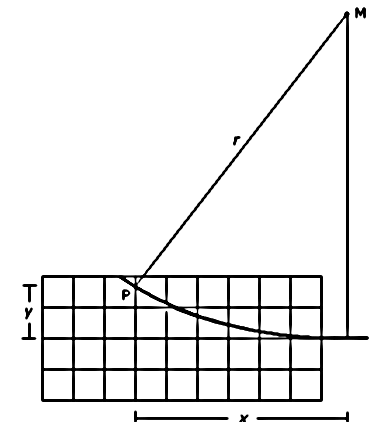
\includegraphics[width=2in]{images/radius.png}
\caption{Geometry of electron's circular path through magnetic field.}
\label{circularpath}
\end{center}
\end{figure}

\section{Preliminary Questions}

\begin{enumerate}
\item Obtain Eq.~\ref{eom} from Eqs.~\ref{energy} and \ref{newton}.
\item Derive Eq.~\ref{circle}.
\item Using the given numerical data, write Eq.~\ref{helmholtz} in the form $B = CI$,
where $C$ is a numerical constant that you can evaluate from Eq.~\ref{helmholtz}.
What are the units of $B$ and $I$? 
\end{enumerate}

\section{Apparatus}

See Figure~\ref{tubepic} to reference the relevant features of the $e/m$ deflection tube:

\begin{enumerate}
\item Fluorescent screen
\item Lower deflection plate (not used)
\item Boss with 4 mm plug for connecting deflection plate (not used)
\item Electron gun
\item 4 mm sockets for connecting heater supply and cathode
\item 4 mm plug for connecting anode (accelerating voltage)
\item Upper deflection plate (not used)
\end{enumerate}

\begin{figure}
\begin{center}
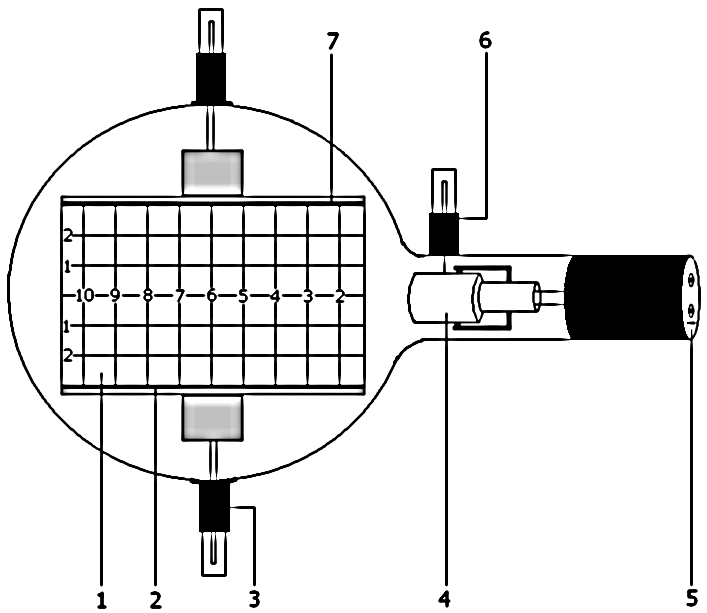
\includegraphics[width=4in]{images/teltron525.png} 
\caption{Location of terminals on Teltron 525 deflection tube.}
\label{tubepic}
\end{center}
\end{figure}



As shown in Fig.~\ref{tubewiring2}, the tube contains four terminals for electrical
connections, two for the AC voltage (6 V) that serves to heat the
filament and two for the DC accelerating voltage $V_a$.
 Note that the two larger receptacles on the base of the tube connect
to AC terminals of the power supply.  The smaller receptacle is to be
connected to the negative DC terminal.  The positive DC voltage
terminal is connected to the plug pointing perpendicular to the tube
axis located near the electron gun.
%The power supply has 6.3 volt terminals for the filament heating current and high voltage terminals for the accelerating voltage.  
The Helmholtz coils have a separate power supply, and should be connected in a series loop containing the power supply, coils, and ammeter. The full circuit diagram is shown in Figure~\ref{tubewiring}.

\begin{figure}
\begin{center}
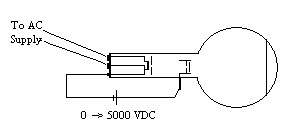
\includegraphics[width=3.0929in,height=1.3543in]{images/ediffraction-img1.png}
\caption{Schematic diagram of electron diffraction tube.}
\label{tubewiring2}
\end{center}
\end{figure}


\begin{figure}
\begin{center}
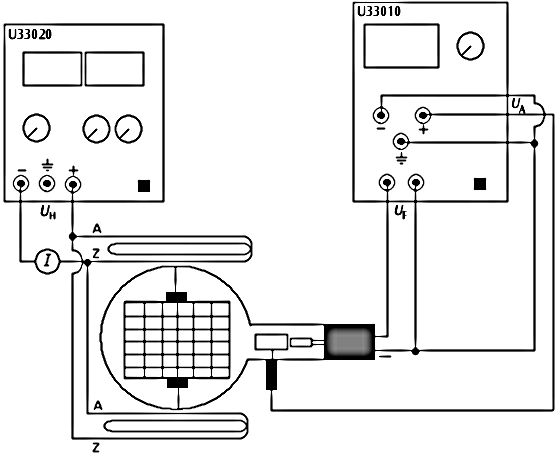
\includegraphics[width=4in]{images/wiring.png} 
\caption{Wiring schematic for Teltron 525 deflection tube.}
\label{tubewiring}
\end{center}
\end{figure}


\section{Procedure}

\textbf{CAUTION}\textbf{: \ High voltages are used in this experiment.
Always slide the high voltage control on the power supply to its lowest
setting before making any changes in the circuit. Have the instructor
check your circuit when you change it before increasing the
voltage.}

\begin{enumerate}
\item Connect the circuit as shown, omitting the electric
field deflection connection,  and with no current running through the
Helmholtz coils. Gradually increase the accelerating voltage until you
see the path of the electron beam on the calibrated fluorescent
screen.



\item Place a bar magnet near the tube to illustrate deflection of the beam. Try various orientations of the bar
magnet. Which gives the largest deflection of the beam?


\item Place the bar magnet perpendicular to the beam with the north pole
nearest to the tube. Using the right hand rule, predict the direction
of the magnetic force on the electrons. Compare to the observed
deflection of the beam.


\item Turn on the Helmholtz coil circuit. Try varying the
magnetic field (by varying the Helmholtz coil current). What is the
effect on the radius of curvature of the electron beam path?

For fixed magnetic field, try varying the accelerating voltage. What is
the effect on the electron beam path radius of curvature?


\item For an accelerating voltage of 2500 volts, adjust the magnetic field
current so that the beam passes through a known point.  For instance, the far corner of the
calibrated region has coordinates $(x,y) =  (10 \rm{cm}, 2.5 \rm{cm})$ . Record the current.


\item Repeat step 5 for larger voltages, incrementing in
steps of 500 volts up to a maximum of 4500 volts.
\end{enumerate}

\section{Analysis}

\begin{enumerate}
\item Explain the results obtained in Procedure steps 1-4 qualitatively
in terms of the appropriate relationships. Hint: for 2 \& 3, consider
the magnetic force law, Eq.~\ref{lorentz}; for step 4, Eq.~\ref{eom} will be helpful.

\item For each set of $V$ and $B$ data taken in Procedure step 5, compute $e/m$
for the electron. Use SI units throughout.

\item Find the mean value of $e/m$ and the uncertainty (standard deviation of
the mean). Compare your results (including the uncertainty) to
$e/m$ as obtained from standard values of $e$ and $m$.
\end{enumerate}

\section{References}
\begin{itemize}
\item Thornton and Rex, Modern Physics, $3^{\rm rd}$ ed., pp. 85-89
\item Equipment instructions: Teltron 525 Deflection Tube
\item Tipler and Llewellan, Modern Physics,$5^{\rm th}$ ed., pp. 116-118
\end{itemize}


\end{document}
